\documentclass[10pt,a4paper]{upmc} 

\usepackage[T1]{fontenc}
\usepackage[utf8]{inputenc}
%\usepackage[english]{babel}
\usepackage{amsmath}
\usepackage{amssymb}
\usepackage[ruled,vlined,linesnumbered]{algorithm2e}
\usepackage{mathtools}
\usepackage[usenames,dvipsnames]{xcolor}
\usepackage{framed}
\usepackage[framemethod=tikz]{mdframed}
\usepackage{listings}         

\global\mdfdefinestyle{graybox}{%
  linecolor=black,linewidth=1pt,%
  backgroundcolor=lightgray
}

\mdfdefinestyle{evaluation}{
    frametitlebackgroundcolor=black!15,
    frametitlerule=true,
    roundcorner=10pt,
    middlelinewidth=1pt,
    innermargin=0.5cm,
    outermargin=0.5cm,
    innerleftmargin=0.5cm,
    innerrightmargin=0.5cm,
    innertopmargin=\topskip,
    innerbottommargin=\topskip,
    frametitle={Evaluation}
}

\framedsolutions
\renewcommand{\solutiontitle}{\noindent\textbf{Solution:}\par\noindent}
\usepackage[textwidth=18cm,textheight=25cm]{geometry}

%\printanswers

\newcommand{\myline}{\noindent\makebox[\linewidth]{\rule{\textwidth}{0.7pt}}}
\newcommand{\mytilde}{\raise.17ex\hbox{$\scriptstyle\mathtt{\sim}$}}
\newcounter{mainmemorder}
\newcommand{\save}{\setcounter{mainmemorder}{\value{enumi}}}
\newcommand{\load}{\setcounter{enumi}{\value{mainmemorder}}}
\newcommand{\mytext}[1]{\colorbox{lightgray}{\texttt{#1}}}
\newcommand{\subsecline}{\texorpdfstring{\hrulefill}{}}
\newcommand{\Num}{Part 2}
\newcommand{\UE}{\scriptsize M1 ISI/SAR/IPS\\ ROS \& experimental robotics}
\renewcommand*{\theenumi}{\#\thesubsection.\arabic{enumi}}
\title{ROS and experimental robotics.\\ \Num: URDF and simulations with ROS}

\lstset{language=matlab,
  basicstyle=\small\sffamily,
  keywordstyle=\color{dblue}\bfseries,  
  commentstyle=\color{dred}\textit,
  stringstyle=\color{dgreen}\ttfamily,
  extendedchars=true,
  frame=single, 
  numbers=left,
  backgroundcolor=\color{lgray}
}

%\setcounter{page}{5}

\begin{document}

\maketitle


\section{ROS tutorial}
\label{sec:tutorial}
\vspace{-0.5cm}\myline\\
After the phase 1 of this teaching unit, you should now master the basic concepts of ROS. The goal
of this second phase is to use these basic skills to program a sensorimotor task for a simulated,
then real, robot. Two tasks will be programmed: the first one corresponds to an essential safety
mechanism, where the robot will have to be able to stop at any time if an obstacle appears in its
path. The second task will be a line following task allowing the robot to automatically follow a
pre-defined path. \\

\noindent In order to perform this kind of elementary tasks, it will be necessary:
\begin{itemize}
  \item to understand and manipulate the universal declaration format that the ROS environment
        proposes to use, i.e.\ the \mytext{URDF} format (Unified Robot Descriptor Format) as well as
        the functioning of \mytext{XACRO} which allows to simplify the writing of this format ;
  \item to understand and exploit the physical simulator we will be using in the following, i.e.\
        \mytext{GAZEBO}.
\end{itemize}
%
\begin{mdframed}[style=graybox]
  The URDF is a ROS specific standardized XML format for representing the model of a robot using
  basic geometries and linkages between them. It allows to have a code-independent, human-readable
  way to describe robots. It takes into account the dynamics of the different parts of the robot and
  their interactions (mechanical linkages, elasticity, viscosity, etc.). An external mesh-file could
  also be associated for display purposes.
\end{mdframed}

As in phase 1, it is mandatory for you to carefully follow the following ROS tutorial as it will
practically explain how \mytext{URDF} and \mytext{XACRO} work together. This thus constitutes a
\textbf{mandatory homework}, and you have about \textbf{2 weeks} to complete the tutorials. In the
meantime, a discussion forum is made available on Moodle and all your teachers will be there to
respond to the questions you might have. \\

\textbf{In the end of the tutorial period, your knowledge and understanding of the \mytext{URDF}
  format and \mytext{Gazebo} simulation will be assessed through multiple choice questions on
  Moodle.}

\begin{mdframed}[style=graybox]
  The tutorial is available at \url{http://wiki.ros.org/urdf/Tutorials} and you have to work on
  the tutorials from the section \textbf{"Learning URDF Step by Step"} :
  \begin{itemize}
    \item Building a Visual Robot Model with URDF from Scratch
    \item Building a Movable Robot Model with URDF
    \item Adding Physical and Collision Properties to a URDF Model
    \item Using Xacro to Clean Up a URDF File
    \item Using a URDF in Gazebo
  \end{itemize}
  \noindent At the end of these tutorials, you are supposed to precisely know:
  \begin{itemize}
    \itemsep=-1pt
    \item the different parts of a Robot description file (URDF file);
          \begin{itemize}
            \item  Geometry description of links
            \item Inertial description
            \item Mechanical description of joints
          \end{itemize}
    \item Basic knowledge about Gazebo and how to make a robot model spawn in a Gazebo simulation

  \end{itemize}
\end{mdframed}
\newpage

\section{Practical teaching}
\vspace{-0.5cm}\myline\\
In this practical teaching, you will successively work on:
%
\begin{itemize}
  \item	the geometrical definition in URDF of a simple robot and the visualization of its geometry
        on \mytext{rviz};
  \item	the exploitation of this description with \mytext{gazebo}, enriched with sensors
        descriptions, to gather sensorimotor data from a (simulated) camera and a laser distance
        sensor;
  \item	the exploitation of the laser data to trigger an ``emergency stop'' behavior in a ROS node;
  \item	some elements of image processing with \texttt{openCV} to program a line following
        algorithm;
  \item	assessing your approach with simulated images coming from \mytext{gazebo} or from a real
        Turtlebot 3 by using the \mytext{rosbag} tool.
\end{itemize}

%\subsection{Objectives}
More precisely, you will first work with RVIZ to visualize an URDF description. You will be able to
modify directly from it the robot joints positions so as to check if this URDF description is
geometrically correct. It can help you in debugging your conception, before actually perform a
physically realistic simulation of the robot.

Next, you will use the physical simulator GAZEBO to simulate the robot dynamic in a realistic --yet
simple-- world. Since the proposed robot is not endowed with exteroceptive sensors, we will add some
of them (a camera and a laser distance sensor) in the robot description to simulate their outputs.
On this basis, you will then be able to program simple sensorimotor skills, like obstacle avoidance
or line following algorithms

Finally, you will be able to assess part of these algorithms on real, recorded data. This will help
you in bridging the gap betwen simulation and real life experiments.

\begin{figure}[!h]
  \centering
  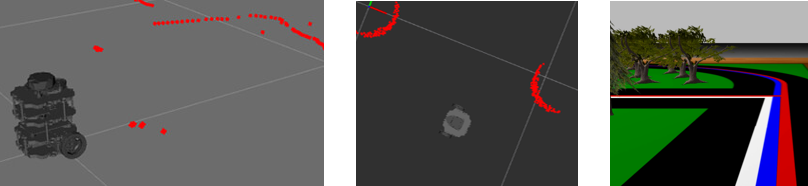
\includegraphics[width=\linewidth]{figures/tache_sensorimotrice.png}
  \caption{Illustration of sensorimotor tasks made with the turtlebot3 Burger}
  \label{fig:turtlebot_family}
\end{figure}

\subsection{Part A: RVIZ \subsecline}
\label{subsec:urdf}

In this first part, you will learn to use a launch file to launch urdf file visualization with RVIZ.

\begin{enumerate}
  \load
  \item Place yourself in the \texttt{src} folder of your ROS workspace, and create a ROS package
        called \texttt{mybot\_description} with a dependency to \texttt{urdf}.

  \item Create a \texttt{launch} folder in your package directory, and put inside the file
        \texttt{rviz.launch} downloaded from Moodle.

  \item Inspect the downloaded launch file and spot where the robot URDF description is defined. Go
        then to the corresponding \mytext{turtlebot3\_description} package and open the URDF
        turtlebot3 description. After the initial URDF tutorial, you should be able to entirely
        understand its content. Do not hesitate to compare the proposed description with the one you
        built during this tutorial. You can also use the \texttt{urdf\_to\_graphiz} instruction to
        better understand the organization of this file.

  \item Read and understand the \texttt{rviz.launch} launch file, then launch it. RVIZ should now
        show up \ldots with an empty window. This is because the robot description must be loaded
        inside RVIZ. \\ To do so, click on the \texttt{Add} button (in the bottom left of the RVIZ
        window), and select the \mytext{RobotModel} within the \texttt{rviz} folder. Comment what is
        happening by reviewing the error messages displayed on RVIZ.

  \item In order to solve the visualization issue, it is first necessary to launch the
        \mytext{joint\_state\_publisher} and the \mytext{robot\_state\_publisher} together with RVIZ.
        Look online to find the exact role of each of these nodes, and add them to the        \texttt{rviz.launch} file accordingly. \\
        Then, launch again RVIZ: does it work correctly now? Inspect again the error
        message and find a solution.

  \item If you close and relaunch RVIZ, you have to systematically add the \mytext{RobotModel}
        visualization. To avoid this, you can backup RVIZ configuration to a file and load it when
        launching RVIZ. To do so, launch RVIZ, and click on \texttt{File -> Save config as}, and
        save RVIZ configuration to a file \texttt{config.rviz} inside a folder \texttt{rviz} inside
        your \mytext{mybot\_description} package. Then, modify the RVIZ launch file to load
        configuration with the \mytext{rviz} node with:\\
        \verb+<node name="rviz" pkg="rviz" type="rviz" args="-d $(find mybot\_description)/rviz/config.rviz"/>+

        \save
\end{enumerate}

Now that the turtlebot3 correctly appears in RVIZ, one will try to make the robot joints actually
move. This can be achieved by publishing adequate messages on the \mytext{/joint\_states}
topic, actually populated by the previously mentioned \mytext{joint\_state\_publisher} node. Instead
of such a \textit{manual} publication, one can also use the \mytext{joint\_state\_publisher\_gui}
node which proposes a graphical interface aiming at controlling through some sliders the different
robot joint positions.

\begin{enumerate}
  \load
  \item Launch the \mytext{joint\_state\_publisher\_gui} node from the \texttt{rviz.launch} file,
        instead of the node \\
        \mytext{\mytext{joint\_state\_publisher}}. A small window should then appear
        together with RVIZ, allowing you to control graphically the robot joints positions.

  \item Move the sliders from this GUI and listen to the messages published on the
        \mytext{/joint\_states} topic. Comment exactly the effect of the
        \mytext{joint\_state\_publisher\_gui} node.

\end{enumerate}

\subsection{Part B: the gazebo simulator}

\indent \mytext{RVIZ} has been used so far only to visualize the geometrical description of our
robot. We will now exploit a physical simulator to put the turtlebot3 robot inside a simulated world
where interactions, dynamics, etc. are properly simulated, allowing a more precise reproduction of
the physical interaction of a real robot in the real world. This will also allow the simulation of
sensory data which will help you in specifying and programming realistic robotics tasks.
%
To do so, one needs to enrich the geometrical purely urdf/xacro robot description with some specific
elements for \mytext{gazebo}, like textures specifications, or motor/joints controllers.

\begin{enumerate}
  \item Inspect again carefully and comment the URDF description of the turtlebot3 burger, and more
        particularly the two included files at the beginning of the file. Explain the role of each.

  \item One now has to "push" the robot inside the simulated world. In ROS, we would say instead
        that the robot has to be "spawned" in the simulated world. To do that, copy the launch file
        \texttt{turtlebot3\_empty\_world} already used at the end of Part 1 in the package
        \mytext{mybot\_teleop} inside a \texttt{launch} folder inside your
        \mytext{mybot\_description} package. Be careful at changing the robot description to the one
        previously used \\(\texttt{turtlebot3\_burger\_for\_autorace\_2020}).
        %
        \begin{enumerate}
          \item Comment the role of the \texttt{<include>} tag by exploring the \mytext{gazebo\_ros}
                package. In particular, explain the role of each parameter and the general structure
                of Gazebo as a server and client.
          \item Then, launch gazebo and spawn the robot with the launch file. Inspect the available
                nodes and topics.
        \end{enumerate}

  \item You can easily add objects in the simulated environment by clicking on the corresponding
        geometric form on the gazebo toolbar. Use now your teleoperation node from Part 1 to
        teleoperate the turtlebot inside \mytext{gazebo} and evaluate the effect of a collision.
  \item Explain how the velocity command is actually used by \mytext{Gazebo} to simulate the robot
        movement by exploring the parameters in the gazebo file included in the URDF description.
  \item Finally, it is often required to simulate the robot with \mytext{gazebo} and to visualize
        all the data available with \mytext{rviz} at the same time. On the basis on the previous
        launch files you created for both tools, create a unique launch file launching both nodes
        together. It will serve as the root basis for all your forthcoming developments.
\end{enumerate}

\subsection{Part C: how to deal with sensors}

All we have done so far is to exploit the geometrical description of the robot and the corresponding
motor controller. A robot is usually also endowed with exteroceptive sensors, which can also be
simulated by Gazebo to obtain realistic data allowing to design and test algorithms in closed loop,
before actually working with real sensory data coming from the actual robot.

\subsubsection{The Laser Distance Sensor}

A Laser Distance Sensor (LDS), or laser rangefinder, is an exteroceptive sensor exploiting a laser
beam to determine the distance to objects in its surrounding environment. Exactly like the motor
controler, the LDS is actually simulated through a gazebo plugin, that must be defined in the
gazebo section/file of the robot description.
%
\begin{enumerate}
  \load
  \item Identify in the Gazebo file of the turtlbot3 description the section devoted to the laser
        sensor. Comment the parameters used in this section (do not hesitate to go to the gazebo
        documentation to find the role of each tag in the LDS definition.)
  \item Spawn the turtlebot in the empty world like before, and add a simple geometrical form in the
        environment. You can then visualize the LDS data directly in Gazebo (\texttt{Window} ->
        \texttt{Topic Visualization}). Observe how they are displayed and how the laser data are modified
        when moving the robot in the environment.
  \item The LDS data are also pushed to ROS on a dedicated topic. List all of the currently active
        topics and find on which topics are published the LDS data, and analyze the message transmitted by
        the simulated LDS sensor.

  \item You can also visualize the laser scans on RVIZ. To do that, select the appropriate
        \texttt{Displays}. Then, teleoperate again the robot to observe the changes in the LDS data.
        Determine the minimum and maximum angles of the LDS measurement directions and the way the
        measurements are gathered in the distance array.

  \item Create a node \mytext{lds\_distance} in a new package \mytext{mybot\_control} that sends on a
        given topic an array of four floats corresponding to the 4 mean values of obstacles detected
        in front, left, right and back of the robot ($\pm 20\deg$) around each direction.

  \item Implement in the \mytext{mybot\_control} package a new node that makes the robot
        automatically stop when facing an obstacle at a distance (which can be manually tuned, for
        instance by using parameters, or services).
    \save
\end{enumerate}

\begin{mdframed}[style=evaluation]
  Call your teacher at the end of this subsection to demonstrate the use of the LDS sensor.
\end{mdframed}

\subsubsection{The camera sensor}
We now have a robot endowed with a working LDS, allowing it to detect obstacles in the environment.
We will now work with the camera mounted on the turtlebot3, which can also be simulated with Gazebo.

\begin{enumerate}
  \load
  \item Following the same steps than with the LDS sensor, comment the section devoted to the camera
        sensor inside the gazebo file, and identify it different parameters and roles.

  \item Spawn a turtlebot3 in \mytext{gazebo} and inspect the available topics. On which topic(s) is
        (are) published the simulated camera? Display the acquired image both on \mytext{gazebo} and
        \mytext{rviz}.
  \save
\end{enumerate}

\subsubsection{The inertial measurement unit}

The turtlebot3 is also endowed with an inertial measurement unit (IMU), which measures and reports
the speed, acceleration and orientation of the robot by using a combination of accelerometers,
gyroscopes, and magnetometers.

\begin{enumerate}
  \load
  \item Follow the exact same steps as before to understand, display and interpret the IMU simulated
        data on Gazebo and RVIZ.
  \save
\end{enumerate}

\subsubsection{Display the sensory data coming from the real turtlbot 3}
The sensory data you displayed on RVIZ were actually simulated by Gazebo and published on their
corresponding topics. But the real sensors, placed on the real turtlebot3, actually send the very
same messages to the same topics, making the visualization of the real sensory data very easy.

\begin{enumerate}
  \load
  \item Follow the procedure to bring up the turtlebot 3 (see in particular the end of part 1 and
        the corresponding ``Turtlbot guide'' on Moodle).
  \item Once operational, list all the available topics from the robot. Launch RVIZ and visualize
        all the sensory data you can from the robot.
  \item Compare the real data with the one simulated by Gazebo. Do you get exactly the same type of
        information? Explain the limitations you might face when prototyping a signal processing algorithm
        on the simulated data.
  \save
\end{enumerate}

\subsection{Part D: a step towards the real robot (\textit{rosbag}) \subsecline}
\label{subsec:rosbag}

The Gazebo simulation, even if it allows to efficiently prototype control laws or basic sensory
processing, does not allow to take into account the variety of conditions encountered with real
systems in the real world. To illustrate this, we will use a ROS tool named \mytext{rosbag} which
aims at recording from and playing back to ROS topics. With \mytext{rosbag}, you can then record all
the data you want during a session on the real robot, and then replay everything so that you can
assess your algorithm against real data in an offline manner. Obviously, this is really useful for
signal processing tests, but can not be used in closed loop conditions.

\begin{enumerate}
  \load
  \item Download from Moodle the file \texttt{turtlebot3.bag} and place it in the virtual machine
        wherever you want on the disc.

  \item Inspect the content of the bag file with the appropriate options of the \mytext{rosbag}
        command. How long is the recording? List all the topics that you can replay from this bag file.
  \item Launch \mytext{rviz} to visualize all the data you can, and play the bag file (note that for
        images, you can also use the \mytext{image\_view} node). Compare qualitatively with the data
        coming from the simulation.
  \item You can also use \mytext{rosbag} to record your own session, be it a simulation or on the
        real robot. Depending on the timing, launch a simulation or the real robot and record your own bag
        file. Try then to replay it.

        \begin{mdframed}[style=evaluation]
          Call your teacher at the end of this subsection to evaluate your work.
        \end{mdframed}

\end{enumerate}

\mytext{rosbag} is a key tool in the projet coming next. You can use it to record e.g.\ images when
teleoperating the robot to calibrate your image processing algorithm, or laser scans to correctly
detect obstacles, etc. That way, you will no longer need to work at 100\% \textbf{on} the real real
robot, while still being able to work \textbf{with} data coming from it. This is the traditional way
to develop algorithms, control laws, etc.\ and it is expected you use it extensively during the
project.

\end{document}

